% --- Insertar en Discussion, sección sugerida: nueva subsección o al final de
%     "Organisational and Socio-Technical Implications" / antes de "Economic
%     Implications and Evidence Gaps" ---

The concentration of the corpus in code quality and technical debt and human--AI interaction (Section 3.1) is not merely a matter of two large, separate literatures. Fig.~\ref{fig:cooccurrence} shows the co-occurrence of analytical dimensions across the binary dimension flags recorded for each study: human--AI interaction and code quality and technical debt co-occur in 175 studies, the single largest off-diagonal cell in the matrix. This indicates that a substantial share of the evidence base treats the reliability of AI-generated code and the dynamics of developer--AI interaction as intertwined phenomena rather than independent research questions, consistent with the socio-technical equilibrium perspective advanced in this study: verification overhead (a CQTD concern) and interaction quality (an HAI concern) are empirically, not just theoretically, coupled.

\begin{figure}[h]
    \centering
    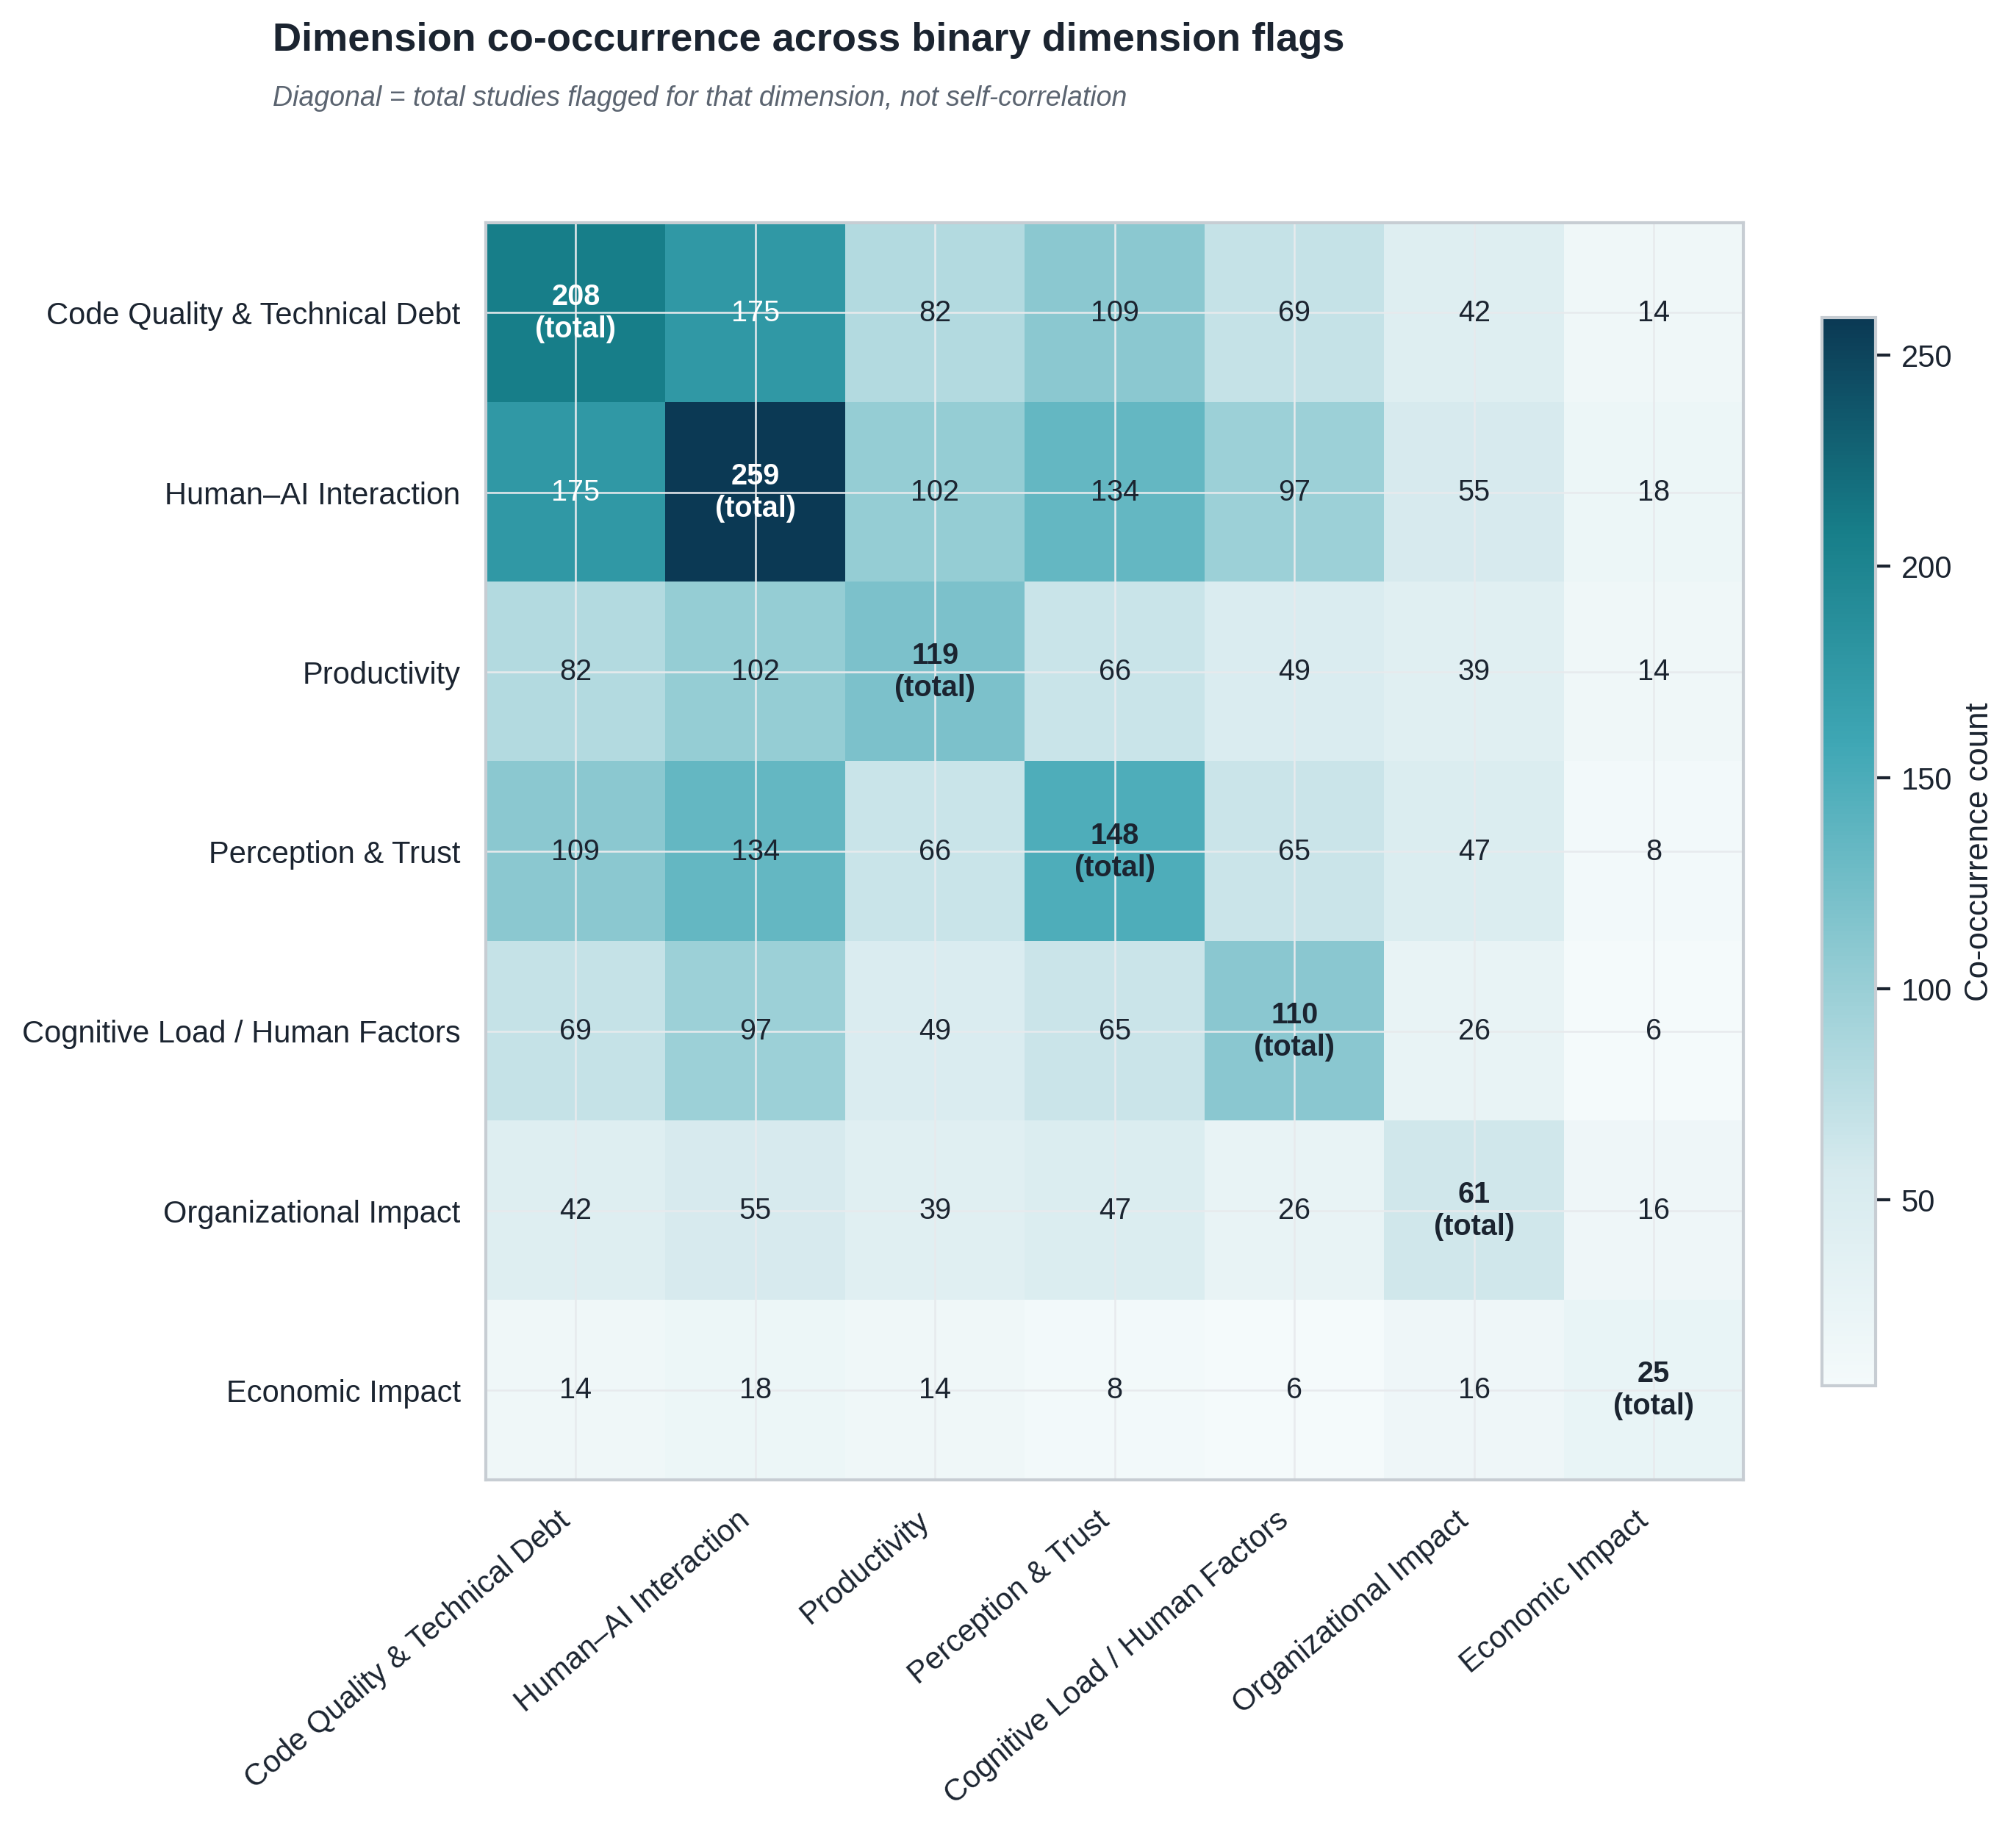
\includegraphics[width=0.82\linewidth]{figures/C1_dimension_cooccurrence.png}
    \caption{Dimension co-occurrence across binary dimension flags. The diagonal reports the total number of studies flagged for that dimension in any role, not self-correlation.}
    \label{fig:cooccurrence}
\end{figure}

This coupling is further reflected in how the methodological rigour of the corpus has evolved. As noted in Section 3.1, the share of A1 (high-rigour) studies rose from 16.7\% in 2022 to 54.7\% in 2026 (Fig.~\ref{fig:quality_evolution}). This trend suggests that the field's growing empirical maturity has accompanied, rather than preceded, its conceptual shift toward treating code quality and human--AI interaction as a joint object of study: as researchers gained more rigorous tools for evaluating AI-generated code, the entanglement between technical reliability and interaction dynamics became increasingly visible in the evidence itself, reinforcing the socio-technical framing proposed in this paper rather than a purely technical one.
